\documentclass[a4paper,10pt]{article}

\title{Serveur domotique}

\author{TERRIE Corentin \\ CROS Bastien \\ MONNIER Matthias}

\date{\today}

\usepackage[utf8]{inputenc}
\usepackage[french]{babel} 
\usepackage{lmodern} % Pour changer le pack de police
\usepackage{makeidx}
\usepackage{fancyhdr}
\usepackage{graphicx}
\usepackage[lofdepth,lotdepth]{subfig}
\usepackage{float}
\usepackage{hyperref}
%---------------------------------------------------------
\usepackage{listings}
\usepackage{textcomp}
% JAVA en couleur ;-)- -----------------------------------
%\lstset{
%language=Java,
%basicstyle=\normalsize, % ou ça==> basicstyle=\scriptsize,
%upquote=true,
%aboveskip={1.5\baselineskip},
%columns=fullflexible,
%showstringspaces=false,
%extendedchars=true,
%breaklines=true,
%showtabs=false,
%showspaces=false,
%showstringspaces=false,
%identifierstyle=\ttfamily,
%keywordstyle=\color[rgb]{0,0,1},
%commentstyle=\color[rgb]{0.133,0.545,0.133},
%stringstyle=\color[rgb]{0.627,0.126,0.941},
%}
%----------------------------------------------------------

\renewcommand{\labelitemii}{$\bullet$}

\begin{document}
\makeatletter
  \begin{titlepage}
  \centering
      {\Large \textsc{École Universitaire Polytechnique de Montpellier}}\\
      \textsc{Microélectronique et Automatique - Électronique et Informatique Industrielle }\\
    \noindent\hrulefill 
    \\
    \vspace{2 cm}
      {\large	\@date\\}
    \vspace{2cm}
       {\huge \textbf{\@title}} \\
	
	\vspace{1cm}
      
\includegraphics[scale=0.15]{head.png}\\

    \vspace{2em}
        {\large \@author} \\
    
    \vspace{2.6cm}
        
\includegraphics[height=0.15\textheight]{mea.jpg}
        \hfill
        
\includegraphics[height=0.15\textheight]{um.png}
  \end{titlepage}
\makeatother
\tableofcontents
\clearpage

%-------------------------------------------------------------------------------------------------------------

\section{Presentation Projet}

-- TITE INTRO --
\begin{figure}[H]
\centering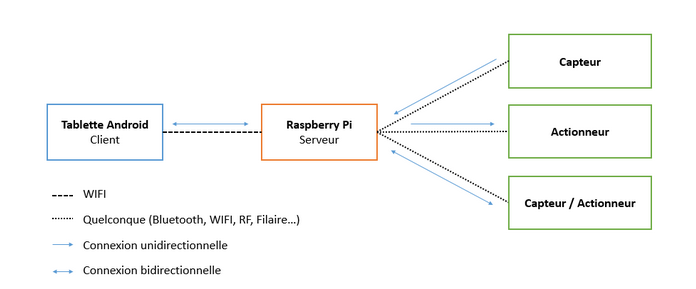
\includegraphics[scale=0.7]{images/Shema_projet.png}
\caption{Schéma montrant les différentes connexion du réseau.}
\end{figure}

%-------------------------------------------------------------------------------

\section{Partie Android (client)}



%-------------------------------------------------------------------------------------------------------------

\section{Partie Raspberry (serveur)}

Le serveur servira a centralisé tout le réseau domotique. Il aura pour tâches : \\
\begin{itemize}
	\item Possibilité de stocker les donnés des capteurs si liaison Tablette-Rasberry coupée.
	\item Gestion des données différentes en fonction de la connexion à un client Android ou un capteur/	actionneur. 
	\item Si connexion à un Android : 
		\begin{itemize}
			\item Envoie des informations concernant les capteurs, les actionneurs, de métrologie, etc. (à définir).
			\item Réception des ordres de la tablette : allumer tel lampe, se connecter à tel capteur, etc. (à définir).
		\end{itemize}
	\item Si connexion à un capteur, simplement lire les informations.
	\item Si connexion à un actionneur, le commander (selon les ordres reçu de la tablette) et gérer son état.
	\item Calcul de métrologie pour chaque connexion.
\end{itemize}

Pour implémenter le serveur, nous avons choisi d'utiliser une Raspberry B+, embarquant un système dérivé de Débian : Raspbian. Cela nous as permit d'implémenter un serveur linux, utilisant les fonctions unix.

\subsection{Première version du serveur : Connexion à un seul client}

Le premier serveur implenter sur la Raspberry permettais seulement de gérer une connexion client/serveur la plus simple possible : le client se connecter grâce au port et l'adresse IP du serveur à celui-ci, et le serveur notifie sur le terminal que la connexion à bien été effectuer. Ensuite le client demande à l'utilisateur de taper quelque chose à l'écran, que le serveur lui renvoi. Finalement le client affiche dans son terminal la réponse du serveur ce qui permet de vérifier que le serveur à bien reçu le message.

Le premier test à été effectuer en implémentant un client linux sur la Raspberry. Ainsi, nous pouvions valider le serveur grâce au client, avant de tester la connexion avec le client Android.

\paragraph{Connexion au client Linux}
%% -> les résultats obtenu, qlq images du terminale, puis les prob rencontré ( problème de buffer)

\paragraph{Connexion avec le client Android}
%% -> les résultats obtenu, qlq images du terminale, puis les prob rencontré ( données pas codé de la même manière)

\subsection{Seconde version du serveur : gestion de plusieurs clients}

\subsection{Troisième version du serveur : échanges de trame au format JSON}

\subsection{Quatrième version du serveur : lancement de tâche différentes selon le type de connexion}
%% -> serveur multi service

%-------------------------------------------------------------------------------------------------------------

\section{Protocoles domotiques}

\subsection{Les protocoles grand public}
%-----
\paragraph{X10}
Le X10 est un vieux protocole (développé en 1975) par courant porteurs.  Les modules X10 peuvent être piloté par des télécommandes radio (433MHz). 

%\underline{\textbf{Les plus :}}
\subparagraph{Les plus :}
\begin{itemize}
\item Protocole le moins cher dans le domaine des automatismes résidentiels
\item Communauté d'utilisateurs très active
\item Bonne distribution des produits
\end{itemize}
\subparagraph{Les moins :}
\begin{itemize}
\item Gros problème de sécurité (toute personne possédant l'accès à une partie de l'installation électrique peut envoyer des ordres X10)
\item Incompatibilité entre les réseaux électriques des différents pays
\item Pas de retour d'état des modules et collisions non gérées
\end{itemize}
Le X10 est vieillissant et par conséquent de nombres constructeurs le délaissent. Il comporte comme seul avantage d'être simple et n'est donc plus conseillé.
%-----
\paragraph{OREGON}
\paragraph{OREGON}


%-------------
\subsection{Les protocoles de rupture technologique}
Deux protocoles seront détaillés dans cette partie : Z-Wave et EnOcean. Ils partagent de nombreuses similitudes, ils sont tous deux :
\begin{itemize}
\item des protocoles domotiques
\item des technologies sans fil
\item des technologies disponibles via plusieurs centrales domotiques
\item des technologies mises en œuvre par plusieurs constructeurs de périphériques.

\end{itemize}
%-----
\paragraph{Z-Wave}
Le Z-Wave est un protocole radio conçu pour la domotique. Il utilise la fréquence $848.42$MHz.
Ses caractéristiques sont qu'il est relativement sécurisé, à double sens (chaque composant est à la fois récepteur et émetteur) et qu'il utilise un réseau maillé.
%\underline{\textbf{Les plus :}}
\subparagraph{Les plus :}
\begin{itemize}
\item Grande richesse fonctionnelle.
\item Topologie maillée du réseau sans fil (contrainte de portée levée car les périphériques relayent les informations entre eux).
\item Retour d'état des périphérique (acquittement de commande, retour d'état de la batterie etc...).
\item Grande liberté de choix sur les périphériques.
\end{itemize}
\subparagraph{Les moins :}
\begin{itemize}
\item Complexité de la mise en place.
\item Prix élevé des modules.
\item Consommateur de pile.\newline
\end{itemize}
Le Z-Wave est un protocole de choix pour les actionneurs mais moins pour les capteurs. Voici le résumé graphique :

%\begin{figure}[H]
%\centering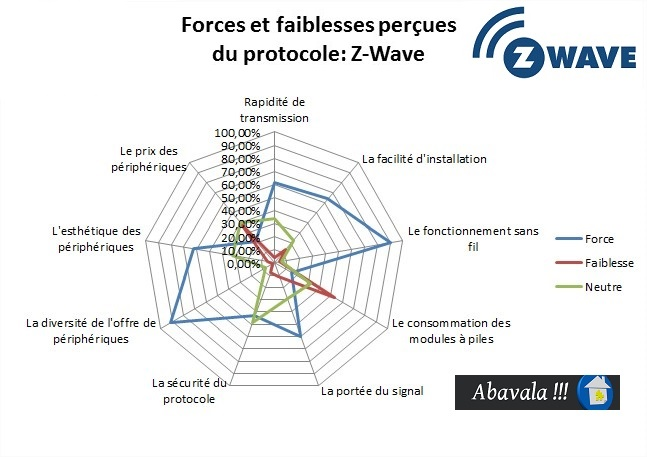
\includegraphics[scale=0.7]{images/forces-protocole-zwave.jpg}
%\caption{Forces et faiblesses du protocole Z-Wave.}
%\end{figure}

%-----
\paragraph{EnOcean}
Le Enocean est également un protocole radio utilisant la fréquence $848.42$MHz. Ce protocole à l'avantage d'être sans fils et sans piles. En effet les périphériques puisent leur source d'énergie de leur environnement direct. Il utilise notamment l'effet photovoltaïque (transforme la lumière en électricité), l'effet piezo-électrique (transforme un choc ou une forte pression en électricité) ainsi que l’effet Peltier ou effet thermoélectrique (transforme une différence de température constaté à un instant donné en électricité).

Lorsqu’un interrupteur EnOcean utilise des cristaux piezo-électrique pour produire son électricité, il communique son ordre ON/OFF par voie hertzienne en utilisant l’énergie fournie par la pression mécanique de celui qui actionne l’interrupteur. Il peut ainsi générer le peu de courant nécessaire pour envoyer l’information à la centrale.

%\underline{\textbf{Les plus :}}
\subparagraph{Les plus :}
\begin{itemize}
\item Flexibilité élevée lors de la mise en oeuvre mais également en cas de modification de l'installation.
\item Pas besoin de changer les piles.
\item Pas de coût de consommables.
\end{itemize}
\subparagraph{Les moins :}
\begin{itemize}
\item Coût des modules plus important que certaines autres technologies.
\item Design peut attrayant de certains modules.
\item Retour d'état non disponible pour certains périphériques (seuls ceux ayant une batterie de stockage de l'énergie le peuvent).
\item Le réseaux n'est pas maillé. Mais il existe des relayeurs graces auxquels le réseaux peut rayonner sur une portée de 200m.\newline
\end{itemize}


Voici le résumé graphique :
%\begin{figure}[H]
%\centering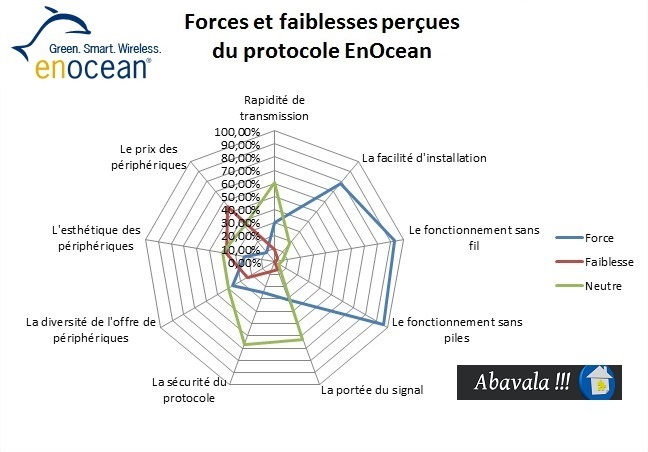
\includegraphics[scale=0.7]{images/forces-protocole-enocean.jpg}
%\caption{Forces et faiblesses du protocole EnOcean.}
%\end{figure}

Les deux graphiques précédent sont issues du site \url{www.abavala.com}. Elles ne sont pas issues de mesures scientifiques mais d’avis personnels exprimés librement. Voici le graphique qui regroupes ces deux protocoles :

%\begin{figure}[H]
%\centering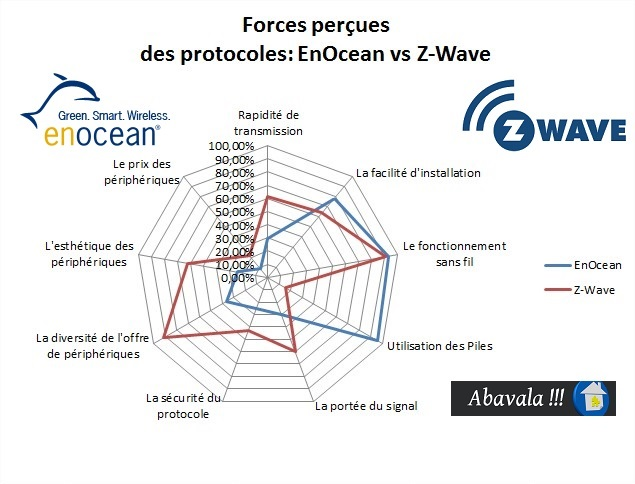
\includegraphics[scale=0.7]{images/forces-enocean-vs-z-wave.jpg}
%\caption{Comparaison des deux protocoles.}
%\end{figure}
%-------------------------------------------------------------------------------------------------------------

\section{Annexes}


 
%-------------------------------------------------------------------------------------------------------------

\end{document}
